\wip
\section{Programm-Entwicklung}
Die für diese Diplomarbeit entwickelte Hardware enthält intelligente Komponenten, die auch programmiert werden müssen.
Diese sind zum einen der bereits vorher existierende \ac{rpi} und der neu hinzugefügte ATMega 328P Mikrocontroller.
\subsection{Mikrocontroller}
\subsubsection{Entwicklungsumgebung}
Die \ac{ide-dev} von Arduino ist eine plattformübergreifende Anwendung (für Windows, MacOS, Linux), die in Funktionen aus C und C++ geschrieben ist.
Sie wird zum Schreiben und Hochladen von Programmen auf Arduino-kompatible Boards, aber auch, mit Hilfe von 3rd-Party-Cores, auf Entwicklungsboards anderer Hersteller verwendet.

Der Quellcode für die \ac{ide-dev} wurde unter der \ac{gnu} \ac{gpl} Version 2, veröffentlicht.
Die Arduino \ac{ide-dev} unterstützt die Sprachen C und C++ unter Verwendung spezieller Regeln der Code-Strukturierung.
Die Arduino \ac{ide-dev} liefert eine Software-Bibliothek aus dem Wiring-Projekt, die viele gängige Ein- und Ausgabeprozeduren zur Verfügung stellt.
Benutzergeschriebener Code benötigt nur zwei grundlegende Funktionen, zum Starten des Sketch und der Hauptprogrammschleife, die kompiliert und mit einem Programmstub main() zu einem ausführbaren zyklischen Ausführungsprogramm mit der \ac{gnu}-Toolchain, die ebenfalls in der \ac{ide-dev}-Distribution enthalten ist, verknüpft werden.
%quelle!!

\subsubsection{Programmierung}
Der in dieser Diplomarbeit verwendete Mikrocontroller besitzt keine \ac{usb}-Schnittstelle, sondern muss über ein externes Programmiergerät mittels \ac{spi}-Schnittstelle programmiert werden.

Als Programmiergerät wurde ein Arduino-Mega-Entwicklungsboard gewählt. Dieses verfügt über eine \ac{icsp}-Schnittstelle, mit der ein anderer Mikrocontroller über \ac{spi} programmiert werden kann. Diese Schnittstelle und deren Pinbelegung ist in Abbildung \ref{fig:icsp-header} dargestellt.
\begin{figure}[htbp!]
    \centering
    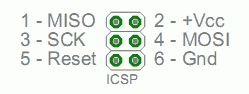
\includegraphics[width=8cm]{images/hardware-programmierung/ICSPHeader.jpg}
    \caption{\ac{icsp} Schnittstelle}
    \label{fig:icsp-header}
\end{figure}

Das Arduino-Board, welches als Programmiergerät verwendet wird, muss mit Hilfe des mitgelieferten Programmes als \ac{isp}-Programmiergerät konfiguriert werden. Das Programm ist in der Arduino \ac{ide-dev} wie in Abbildung \ref{fig:arduino-isp-sketch} dargestellt zu finden.
\begin{figure}[htbp!]
    \centering
    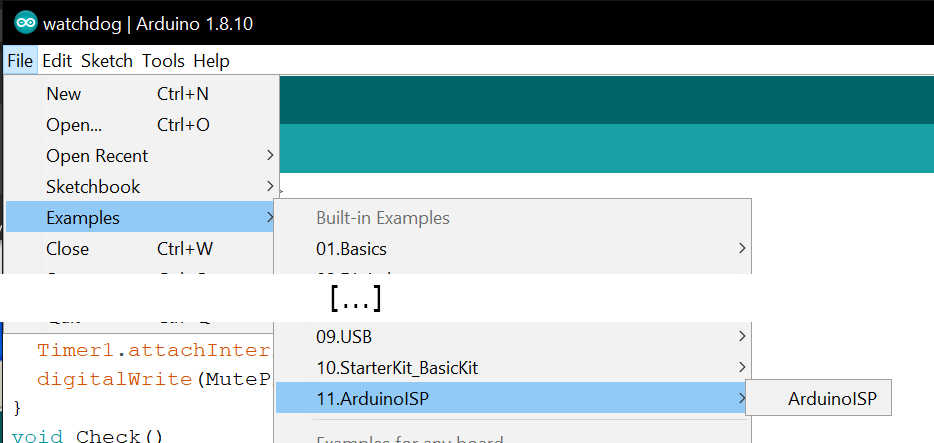
\includegraphics[width=.9\linewidth]{images/hardware-programmierung/arduino-isp-sketch.png}
    \caption{ArduinoISP Sketch}
    \label{fig:arduino-isp-sketch}
\end{figure}

Bevor das eigentliche Programm auf den Mikrocontroller der Station hochgeladen werden kann, müssen noch ein paar Einstellungen in der Arduino \ac{ide-dev} getroffen werden (siehe auch Abbildung \ref{fig:arduino-options}):
\begin{itemize}
    \item Arduino/Genuino Uno als Board auswählen (Dieses Board wird standardmäßig mit dem hier verwendeten Mikrocontroller ausgeführt)
    \item Auswahl der Schnittstelle, an welche das Programmiergerät angeschlossen ist.
    \item Die Option \enquote{Programmer} muss von \enquote{AVRISP mkII} auf \enquote{Arduino as ISP} umgestellt werden.
\end{itemize}
\begin{figure}[htbp!]
    \centering
    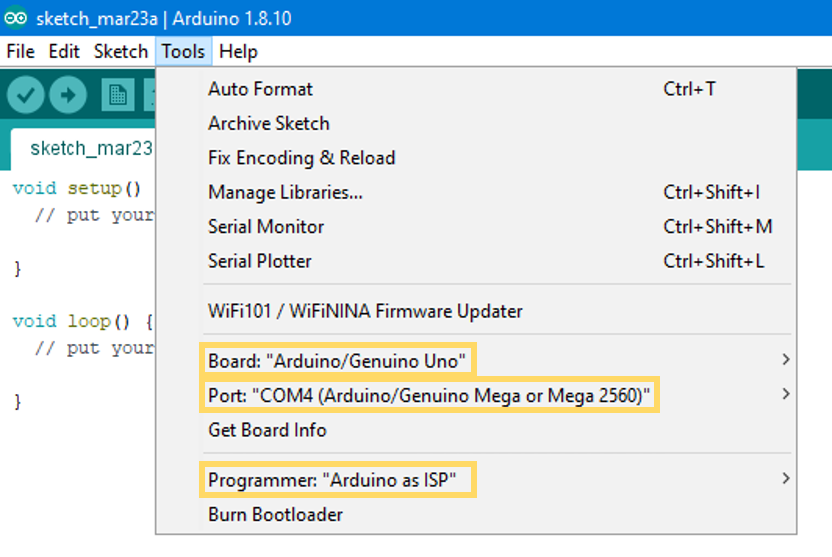
\includegraphics[width=.9\linewidth]{images/hardware-programmierung/optionen.png}
    \caption{Arduino \ac{ide-dev} Einstellungen}
    \label{fig:arduino-options}
\end{figure}

Um nun den Upload-Prozess zu starten muss in der Arduino \ac{ide-dev} \enquote{Upload using Programmer} ausgewählt werden (siehe Abbildung \ref{fig:arduino-upload}).
Das Mikrocontroller-Programm wird nun kompiliert und mit Hilfe des Programmiergerätes auf den Mikrocontroller geladen.
\begin{figure}[htbp!]
    \centering
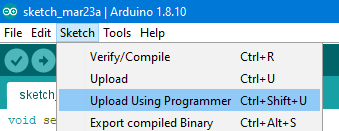
\includegraphics[width=.7\linewidth]{images/hardware-programmierung/upload.png}
    \caption{Hochladen des Programmes}
    \label{fig:arduino-upload}
\end{figure}

\subsubsection{Programm-Dokumentation}
Der Mikrocontroller wird in C++ mit vorgefertigten Funktionen von Arduino programmiert.

\begin{minted}[firstnumber=1]{arduino}
#include <TimerOne.h>
const int ResetPin = 2, MutePin = 3, SecurityPin = 4;
volatile bool FindEnable = false;
bool Reboot = true;
\end{minted}
\paragraph{1:}
Die TimerOne Bibliothek ermöglicht die Verwendung der Intrerrupt-Funktion des Hardware-Timers des Mikrocontrollers, wodurch das periodische Aufrufen einer Funktion vereinfacht wird.
Dies dient dem ständigen Abfragen des Betriebszustandes des \ac{rpi}.

\paragraph{2:}
Hier werden die verwendeten Pin-Nummern des Mikrocontrollers in Konstanten gespeichert, um das Programm lesbar zu halten.
Zu beachten ist, dass die Nummern des Programms nicht mit den physikalischen Pin-Nummern übereinstimmen.
Das liegt daran, dass die Zuordnung auf einem Arduino-Entwicklungs-Board basiert.

\paragraph{3-4:}
Weiters werden alle globalen Variablen definiert.
Das volatile-Schlüsselwort wird gebraucht, wenn die Variable in einer Interrupt Service Routine verändert wird.
Das Schlüsselwort hat zur Wirkung, dass der Wert der Variable nicht zwischengespeichert, sondern immer der aktuelle Wert abgerufen wird.
Dies ist notwendig, da die \ac{isr} den Programmablauf jederzeit unterbrechen und den Wert zu einem ungünstigen Zeitpunkt verändern kann.

\begin{minted}[firstnumber=6]{arduino}
void setup()
{
    pinMode(ResetPin, OUTPUT);
    pinMode(MutePin, OUTPUT);
    pinMode(SecurityPin, INPUT);
    
    Serial.begin(9600);
    Serial.setTimeout(1000);
    Timer1.initialize(10000000);
    Timer1.attachInterrupt(Check);
    digitalWrite(MutePin, HIGH);
}
\end{minted}
Die Setup-Funktion wird einmalig nach dem Start bzw. Reset des Mikrocontrollers aufgerufen. In dieser werden meist Initialisierungen durchgeführt.

\paragraph{8-10:}
Mit pinMode() wird festgelegt, ob ein \ac{io}-Pin als Ausgang oder als Eingang konfiguriert ist.

\paragraph{12-13:}
Die serielle \ac{uart}-Schnittstelle kann mit dem Serial-Objekt manipuliert werden.
Zum Initialisieren muss die Übertragungsrate in Bit/s angegeben werden, da \ac{uart} keine Taktleitung hat.
Weiters wird das Timeout auf 1 Sekunde gesetzt.
Die Serial.find()-Funktion, welche im Hauptteil verwendet wird, versucht so lange eine Zeichensequenz in der Datenübertragung zu finden, bis das Timeout abgelaufen ist.

\paragraph{14-15:}
An dieser Stelle wird die TimerOne-Bibliothek initialisiert.
Zuerst wird die Periodendauer zwischen den Interrupts in µs definiert.
10 Sekunden sind für diese Anwendung ausreichend schnell, während die Schnittstelle nicht unnötig viel verwendet wird.
Mit attachInterrupt() kann die Funktion für die \ac{isr} definiert werden.

\paragraph{16:}
Mit digitalWrite kann der Zustand eines digitalen Ausgangs festgelegt werden.
Hier wird der Ausgang, welcher den Lautsprecher-Verstärker abschaltet, auf logisch 1 gesetzt.
Dies verhindert etwaige Störgeräusche am Lautsprecher, wenn dieser nicht gebraucht wird.
Der \ac{rpi} kann mit einem Befehl über die \ac{uart}-Schnittstelle den Lautsprecher freigeben.
Dies ist allerdings noch nicht vollständig implementiert.

\begin{minted}[firstnumber=19]{arduino}
void Check()
{
    FindEnable = true;
}
\end{minted}

\paragraph{19-22:}
Die \ac{isr} sollte generell sehr kurz gehalten werden, da sie den normalen Programmablauf unterbricht.
Funktionen der seriellen Kommunikation werden deswegen hier nicht verwendet.
Stattdessen wird eine Variable gesetzt, welche im Hauptprogramm einen alternativen Ausführungszweig auslöst.
Wichtig ist, dass die Variable wie oben bereits beschrieben als volatile deklariert wurde.

\begin{minted}[firstnumber=24]{arduino}
void loop()
{
    if (FindEnable && !Reboot)
    {
        Serial.write("Hello\n");
        FindEnable = false;
        if (Serial.find("Imthere"))
        {
            digitalWrite(ResetPin, LOW);
        }
        else
        {
            Reboot = true;
            digitalWrite(ResetPin, HIGH);
            delay(1000);
            digitalWrite(ResetPin, LOW);
        }
    }
    else if (Reboot)
    {
        if (Serial.find("Rebooted"))
        {
            Reboot = false;
            FindEnable = false;
        }
    }
\end{minted}
Die Loop Funktion ist eine Endlosschleife, in welcher sich die Hauptfunktionalität des Programms befindet.

\paragraph{26:}
Die erste if-Abfrage stellt fest ob der Watchdog seine Überprüfung durchführen soll.
Als Bedingungen für eine Überprüfung des \ac{rpi} sind hier definiert, dass der \ac{rpi} nicht gerade neustartet und die Watchdog-Zeit abgelaufen ist.

\paragraph{28-40:}
Die Überprüfung wird durchgeführt.
Der Mikrocontroller sendet „Hello\textbackslash n“ (\textbackslash n signalisiert das Ende der Übertragung) und wartet auf die Antwort „Imthere“ des \ac{rpi}.
Nach 1000ms ohne Antwort setzt der Mikrocontroller den \ac{rpi} mit Hilfe des Reset-Pins zurück.
Zusätzlich wird die Variable Reboot gesetzt, um den \ac{rpi} nicht während dem Neustarten erneut zurückzusetzen.

\paragraph{42-49:}
Die else if Anweisung sorgt beim Neustart des \ac{rpi} für Schutz vor ungewolltes Rücksetzen.
Die Rebooted-Variable wird erst dann wieder zurückgesetzt, wenn der \ac{rpi} die Nachricht „Rebooted“ schickt.
Diese signalisiert, dass der \ac{rpi} vollständig hochgefahren ist und auf weitere Anfragen reagieren kann.

\begin{minted}[firstnumber=51]{arduino}
    if (Serial.available())
    {
        if (Serial.find("Imclosing"))
            Reboot = true;
        if (Serial.find("Enable"))
            digitalWrite(MutePin, HIGH);
        if (Serial.find("Disable"))
            digitalWrite(MutePin, LOW);
    }
    //---------------------------------
    if (digitalRead(SecurityPin))
        Serial.write("Securitybreached");
}
\end{minted}

\paragraph{51-59:}
Innerhalb dieser if-Abfrage wird auf sonstige Ereignisse, die der \ac{rpi} auslösen kann reagiert.
Wenn der \ac{rpi} neustartet, sendet er die Nachricht „Imclosing“ and den Mikrocontroller, damit dieser den Watchdog-Timer temporär ausschaltet.
Mit „Enable“ und „Disable“ kann der \ac{rpi} den Lautsprecher-Verstärker ein- bzw. ausschalten.

\paragraph{61-62:}
Als letztes wird die Diebstahlsicherung für eine Station über den Mikrocontroller gesteuert.
Falls die Diebstahlsicherung anschlägt wird zum \ac{rpi} eine Nachricht übermittelt, dass dieser entsprechend reagiert.

\subsection{Raspberry Pi}
